\subsectionold{x86}

\subsubsectionold{\NonOptimizing MSVC}

We get (MSVC 2010):

\lstinputlisting[caption=MSVC 2010]{patterns/14_bitfields/2_set_reset/set_reset_msvc.asm}

\myindex{x86!\Instructions!OR}

The \OR instruction sets one bit to value while ignoring the rest.

\myindex{x86!\Instructions!AND}

\AND resets one bit. It can be said that \AND just copies all bits except one.
Indeed, in the second \AND operand only the bits that need to be saved are set,
just the one do not want to copy is not (which is 0 in the bitmask).
It is the easier way to memorize the logic.

\clearpage
\myparagraphold{\olly}

Let's try this example in \olly.

First, let's see the binary form of the constants we are going to use:

\TT{0x200} (0000000000000000000{\color{red}1}000000000) (i.e., the 10th bit (counting from 1st)).

Inverted \TT{0x200} is \TT{0xFFFFFDFF} (1111111111111111111{\color{red}0}111111111).

\TT{0x4000} (00000000000000{\color{red}1}00000000000000) (i.e., the 15th bit).

The input value is: \TT{0x12340678} (10010001101000000011001111000).
We see how it's loaded:

\begin{figure}[H]
\centering
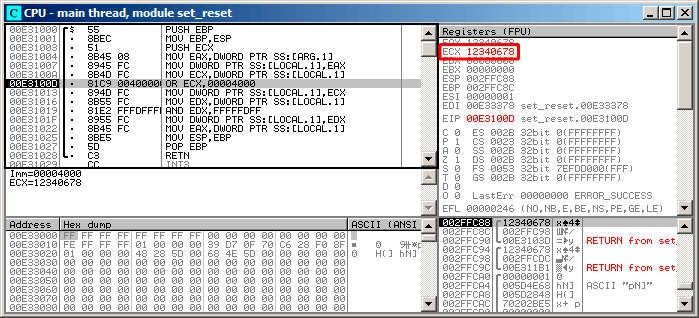
\includegraphics[scale=\FigScale]{patterns/14_bitfields/2_set_reset/olly1.png}
\caption{\olly: value is loaded into \ECX}
\label{fig:set_reset_olly1}
\end{figure}

\clearpage
\OR got executed:

\begin{figure}[H]
\centering
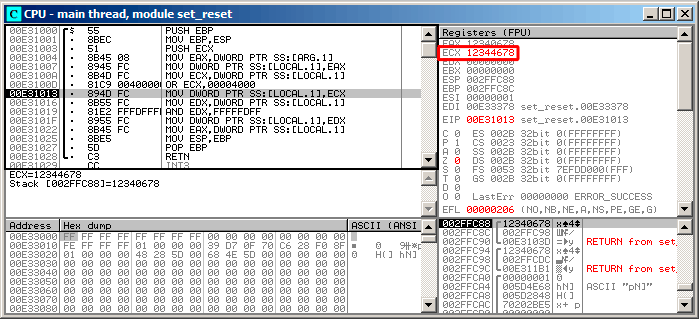
\includegraphics[scale=\FigScale]{patterns/14_bitfields/2_set_reset/olly2.png}
\caption{\olly: \OR executed}
\label{fig:set_reset_olly2}
\end{figure}

15th bit is set: \TT{0x1234{\color{red}4}678} 
(10010001101000{\color{red}1}00011001111000).

\clearpage
The value is reloaded again (because the compiler is not in optimizing mode): 

\begin{figure}[H]
\centering
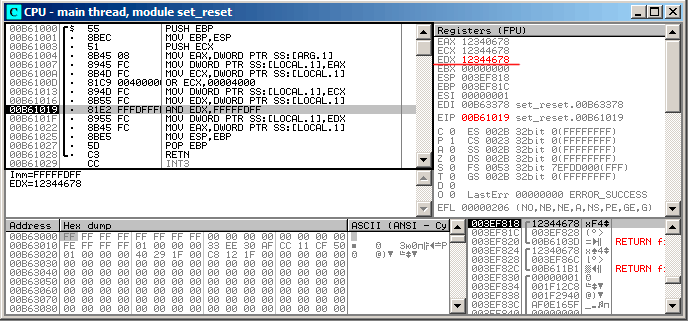
\includegraphics[scale=\FigScale]{patterns/14_bitfields/2_set_reset/olly3.png}
\caption{\olly: value was reloaded into \EDX}
\label{fig:set_reset_olly3}
\end{figure}

\clearpage
\AND got executed:

\begin{figure}[H]
\centering
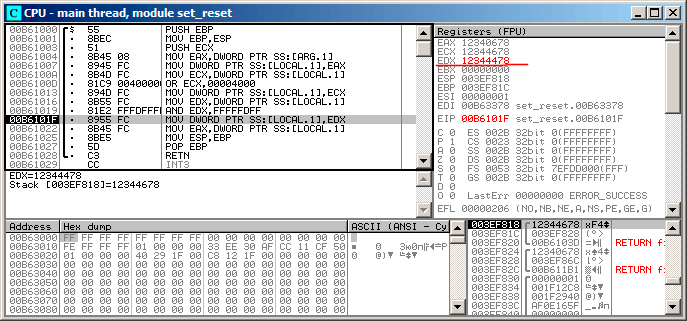
\includegraphics[scale=\FigScale]{patterns/14_bitfields/2_set_reset/olly4.png}
\caption{\olly: \AND executed}
\label{fig:set_reset_olly4}
\end{figure}

The 10th bit was cleared (or, in other words, all bits were left except the 10th) and the final value now is \\
\TT{0x12344{\color{red}4}78} (1001000110100010001{\color{red}0}001111000).

\subsubsectionold{\Optimizing MSVC}

If we compile it in MSVC with optimization turned on (\Ox), the code is even shorter:

\lstinputlisting[caption=\Optimizing MSVC]{patterns/14_bitfields/2_set_reset/set_reset_msvc_Ox.asm}

\subsubsectionold{\NonOptimizing GCC}

Let's try GCC 4.4.1 without optimization:

\lstinputlisting[caption=\NonOptimizing GCC]{patterns/14_bitfields/2_set_reset/set_reset_gcc.asm}

There is a redundant code present, however, it is shorter than the MSVC version without optimization.

Now let's try GCC with optimization turned on \Othree:

\subsubsectionold{\Optimizing GCC}

\lstinputlisting[caption=\Optimizing GCC]{patterns/14_bitfields/2_set_reset/set_reset_gcc_O3.asm}

That's shorter.
It is worth noting the compiler works with the \EAX register part via the \AH register---that is the \EAX register part from the 8th to the 15th bits included.

\RegTableOne{RAX}{EAX}{AX}{AH}{AL}

\myindex{Intel!8086}
\myindex{Intel!80386}
N.B.  The 16-bit CPU 8086 accumulator was named \AX and consisted of two 8-bit 
halves---\AL (lower byte) and \AH (higher byte).
In 80386 almost all registers were extended to 32-bit, the accumulator was named \EAX, 
but for the sake of compatibility,
its \IT{older parts} may be still accessed as \AX/\AH/\AL.

Since all x86 CPUs are successors of the 16-bit 8086 CPU, these \IT{older} 16-bit opcodes are shorter 
than the newer 32-bit ones.
That's why the \INS{or ah, 40h} instruction occupies only 3 bytes.
It would be more logical way to emit here \INS{or eax, 04000h}
but that is 5 bytes, or even 6
(in case the register in the first operand is not \EAX).

\subsubsectionold{\Optimizing GCC and regparm}

It would be even shorter if to turn on the \Othree optimization flag and also set \TT{regparm=3}.

\lstinputlisting[caption=\Optimizing GCC]{patterns/14_bitfields/2_set_reset/set_reset_gcc_O3_regparm3.asm}

\myindex{Inline code}

Indeed, the first argument is already loaded in \EAX, so it is possible to work with it in-place.
It is worth noting that both the function prologue (\INS{push ebp / mov ebp,esp}) and epilogue (\INS{pop ebp})
can easily be omitted here, but GCC probably is not good enough to do such code size optimizations.
However, such short functions are better to be \IT{inlined functions} (\myref{inline_code}).
